\section{Marco Teórico}

\subsection{Internet de las Cosas}

La internet de las cosas es un sistema de dispositivos de computación interrelacionados, máquinas mecánicas y digitales, objetos, animales o personas que tienen identificadores únicos y la capacidad de transferir datos a través de una red, sin requerir de interacciones humano a humano o humano a computadora. \\

Kevin Ashton explica el potencial del internet de las cosas así: ``...El problema es que la gente tiene tiempo, atención y precisión limitados, lo que significa que no son muy buenos para capturar datos sobre cosas en el mundo real. Si tuviéramos computadoras que supieran todo lo que hay que saber acerca de las cosas –utilizando datos que recopilaron sin ninguna ayuda de nosotros– podríamos rastrear y contar todo, y reducir en gran medida los desechos, las pérdidas y el costo. Sabríamos cuándo necesitamos reemplazar, reparar o recordar cosas, y si eran frescas o ya pasadas”. \cite{Asthon2009} 

\subsection{Smart House}

El concepto de Smart House implica tres características básicas. En primer lugar, el monitoreo a través de redes de sensores para obtener información sobre la casa y sus residentes. En segundo lugar, los mecanismos que controlan el uso de la comunicación entre dispositivos con el fin de permitir la automatización y el acceso remoto. Por último, las interfaces de usuario, como los teléfonos inteligentes y las computadoras que permiten a los usuarios especificar las preferencias, así como presentar información a las personas acerca de estas. \\

\subsubsection{Plataforma Heroku}

``Heroku es una plataforma en la nube basada en un sistema gestionado por contenedores, con servicios de datos integrados y un potente ecosistema para desarrollar y ejecutar aplicaciones modernas. La experiencia de los desarrolladores de Heroku es un enfoque centrado en aplicaciones para la entrega de software, integrado con las herramientas y flujos de trabajo de desarrollador más populares de la actualidad'' \cite{Hero}.\\


\subsubsection{Framework Laravel}

``Laravel es un framework de aplicaciones web con una sintaxis expresiva y elegante. Laravel intenta aliviar el dolor del desarrollo al facilitar las tareas comunes que se utilizan en la mayoría de los proyectos web, como la autenticación, el enrutamiento, las sesiones y el almacenamiento en caché.\\

Laravel es accesible, pero potente, y proporciona potentes herramientas necesarias para aplicaciones grandes y robustas. Una magnífica inversión de contenedores de control, un sistema de migración expresivo y un soporte de prueba de unidades estrechamente integrado le brindan las herramientas que necesita para construir cualquier aplicación'' \cite{Lara}. \\

\subsubsection{JSON}

``JSON (JavaScript Object Notation - Notación de Objetos de JavaScript) es un formato ligero de intercambio de datos. Leerlo y escribirlo es cómodo para los humanos, al igual que para las máquinas resulta simple interpretarlo y generarlo. Está basado en un subconjunto del Lenguaje de Programación JavaScript, Standard ECMA-262 3rd Edition - Diciembre 1999. JSON es un formato de texto que es completamente independiente del lenguaje pero utiliza convenciones que son ampliamente conocidos por los programadores de la familia de lenguajes C, incluyendo C, C++, C\#, Java, JavaScript, Perl, Python, y muchos otros. Estas propiedades hacen que JSON sea un lenguaje ideal para el intercambio de datos'' \cite{JSON}.

\subsection{Hardware}

\subsubsection{ESP-WROOM-32}

Es un potente módulo MCU Wi-Fi + BT + BLE que se dirige a una amplia variedad de aplicaciones, desde redes de sensores de baja potencia hasta las tareas más exigentes, como codificación de voz, transmisión de música y decodificación de MP3, además de su reducido tamaño, según se observa en la figura \ref{fig:esp32-wroom-s32-00}.\\

El sistema operativo elegido para ESP32 es freeRTOS con LwIP; TLS 1.2 con aceleración de hardware está integrado también, además se admite la actualización segura (cifrada) a través del aire (OTA), de modo que los desarrolladores puedan actualizar continuamente sus productos incluso después de su lanzamiento.\cite{EW32}\\

%\begin{figure}[H]
%	\centering
%	\caption{ESP WROOM 32. Tomado de: \cite{ESPIMG}}
%	\label{fig:esp32-wroom-s32-00}
%	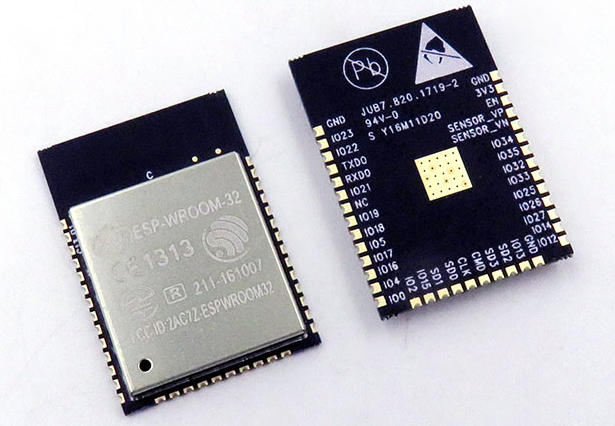
\includegraphics{Imagenes/esp32-wroom-s32-00}
%\end{figure}

\subsubsection{Control de potencia AC por ángulo de fase}

``Los SCR y los TRIAC, permiten aplicar una técnica muy conveniente y eficaz para controlar el voltaje promedio y por lo tanto la potencia aplicada a una carga, cambiando el ángulo de fase con el cual la fuente de voltaje se aplica a ésta, tal como se muestra en la figura \ref{fig:triacgraph}. Esta técnica de control de voltaje es muy usada en las aplicaciones de regulación de motores, iluminación y temperatura, por ser el voltaje la variable principal en estos tres procesos''.\cite{CEKIT}\\


%\begin{figure}[H]
%	\centering
%	\caption{Representación gráfica del ángulo de disparo y de conducción del TRIAC y de la carga. Tomado de: \cite{CEKIT}.}
%	\label{fig:triacgraph}
%	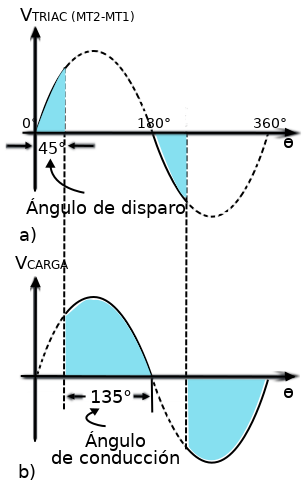
\includegraphics[width=0.3\linewidth]{Imagenes/TRIAC_graph}
%\end{figure}

\subsubsection{Control de Cargas DC}

Los transistores como switch permiten controlar las cargas de corriente continua típicas como los motores y LED's, a parte de poder funcionar en dos estados, encendido y apagado Este control se da mediante la modulación por ancho de pulso (PWM), ya que al variar el ancho de pulso de la señal eléctrica se modifica la cantidad de energía entregada a la carga, tal como se muestra en la figura \ref{fig:pwm-duty-800x396}. \cite{PWM}

%\begin{figure}[H]
%	\centering
%	\caption{Ciclo Útil PWM. [Imagen Propia] }
%	\label{fig:pwm-duty-800x396}
%	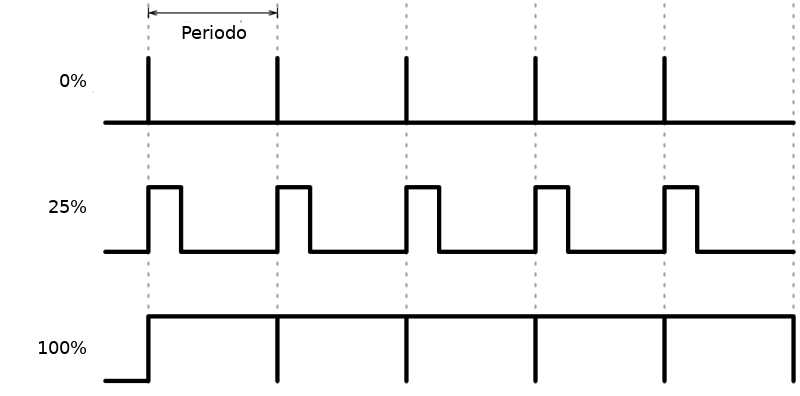
\includegraphics[width=0.5\linewidth]{Imagenes/pwm}
%\end{figure}

\subsection{Software}

\subsubsection{RTOS}

Los sistemas operativos en tiempo real, tienen como parámetro clave al tiempo, ya que en gran variedad de situaciones, por ejemplo, un proceso industrial, se requiere recolectar múltiples datos, los cuales son usados para el control de diversos procesos que deben ser ejecutados en determinados instantes, de no ser así, podría causar desde la mala ejecución de una tarea, hasta un accidente según la delicadeza del proceso.\\ 

Los sistemas de computadoras de bolsillo y los sistemas integrados están diseñados para los consumidores, mientras que los sistemas en tiempo real son más adecuados para el uso industrial. Sin embargo, tienen ciertas características en común''. \cite{SO}\\

\subsubsection{ESP-IDF}

ESP-IDF es el entorno de desarrollo oficial para el ESP32 desarrollado por Espressif System, el cual mediante una serie de comandos específicos escritos en la terminal (en el caso de linux), habilita la configuración del ESP32 en cuanto a su funcionamiento, es decir, permite encender o apagar características como el WiFi, el Bluetooth o realizar particiones de memoria, ademas de esto, se puede cargar el código por el puerto USB al ESP32, al igual que visualizar la información generada por el ESP32 por el mismo puerto. \cite{ES}